\chapter{%
序論}

% 章アブストラクト
配管は気体,液体,粉粒対などの流体を輸送や配線の保護などを目的とする管のことである.
配管は電気配線やケーブルを保護する電気配管や,生活に必要な水を家庭や学校などに輸送する水道管など様々な場面で使用されており,私達の生活において重要な役割を担っている.
そのため,配管を運用するにあたって常に耐久性と安全性を保ち続ける必要性がある. \\

\section{研究背景}
 BIM とは,Building Information Modeling の略称で,コンピュータ上に建築物や土木構造物などの立体モデルを形成し,設計から維持管理までのプロセスをデジタル化する新しいワークフローの一環である.
このBIMモデリングはこれまでの3Dモデリングとは大きく異なる.従来の3次元モデリングでは平面図などの2次元上で作成した図面を元に別途3次元のモデルを作成していた.
そのため,図面と3次元モデルが連動しておらず,設計変更がある度に図面と3Dモデルの両方を修正する必要があり効率的ではなかった.
しかし,このBIM手法は一つのデータを修正すると全てのデータが連動し,関係する図面の該当箇所が自動修正され,従来の方法よりも高校率で作業を行うことが可能になる.\\
 配管は建築物の中でも日常生活に欠かせない存在である.生活に必要な物資を運用したり電線やケーブルを保護するために使用されるなど幅広い面で活用されているため常に耐久性と安全性が求めらている.
その配管の図面を作成する際にはアイソメトリック(アイソメ)図と呼ばれる立体を斜めから見た視点で表示した等角図が用いられる.
このアイソメ図の最大の特徴が図面を見るだけで配管のルートを一目でイメージしやすくなることだ.設計図には平面図や立体図,系統図など
様々な種類の図面を使用するが,配管の場合,配管同士が複数にも重なり合っているため左右上下からの視点では見分けることが困難である.そのため,アイソメ図は図面を立体的に描画する手法を扱えるだけでなく,
配管のルートや交差する配管の前後関係をイメージしやすくなる.\\
\begin{figure}[htbt]
	\centering
	 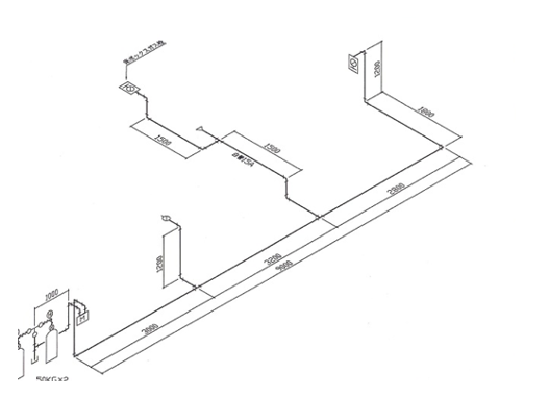
\includegraphics[height=75mm]{Figure/ex_iso.eps}
	 \caption{アイソメ図の例}
	 \label{fig:f1}
\end{figure}

アイソメ図を取得するためにはこれまでにLight Detection and Ranging(LIDAR)センサーと呼ばれるレーザー光を使用して離れた場所にある物体の形状や距離を測定できるセンサーを使用していた.
LIDARセンサーは距離情報を活用して3次元情報を取得するだけでなく,測定範囲の広さや取得データの精度が評価されている.しかしその反面,他のセンサーと比較すると高価であるというデメリットを抱えているため,たくさんの人が
使用することは困難であるとされていた.このような背景から近年LIDARセンサーよりも安価なRGBカメラやRGB-Dカメラを用いた認識手法が研究され始めている.
近年の画像認識分野の研究では機械学習を用いた研究が多く取り上げられている.業務効率化や生産性向上,そして人手不足解消を実現できるというメリットがあり,人工知能の導入は加速していくことが予測されている.

% \begin{figure}[htbt]
% 	\centering
% 	 \includegraphics[height=95mm]{flow.eps}
% 	 \caption{従来のアイソメ図取得方法}
% 	 \label{fig:f2}
% \end{figure}

\section{既存研究}
近年、機械学習を用いた物体認識分野では、6D姿勢推定問題に取り組む研究が盛んに行われている。
この問題では、3次元空間上の位置情報(X, Y, Z)だけでなく、回転や向き(Roll, Pitch, Yaw)も求める必要がある。
物体の姿勢を正確に推定できれば、配管の向きを把握することが可能となり、アイソメ図作成において大きな利点をもたらす。

6D姿勢推定にはRGBカメラやRGB-Dカメラを用いる方法があり、それぞれ異なる特徴と利点がある。
RGBカメラを使用する手法の一例として、6D姿勢推定ネットワーク「Generalizable Model-Free 6-DoF Object Pose Estimation from RGB Images(Gen6D)」を紹介する。
このモデルでは、データセットの作成に「Colmap」というソフトウェアが用いられている。
Colmapは「Structure from Motion(SfM)」技術を用いて、複数の視点から撮影された画像を基に3次元形状を復元するものであり、その結果得られる点群データを基に6D姿勢推定を行う。

Gen6Dの処理は大きく3つのステップに分かれている。
まず「Detector」では、参照画像の情報を基に検出対象物体の領域を特定する。
次に「Selector」では、検出された領域に対応する画像の中から、テスト画像に最も近い視点を持つ参照画像を1枚選び出す。
この参照画像の視点を基に、物体の初期姿勢を形成するが、ここでは多少の誤差が生じる可能性がある。
最後のステップでは、初期姿勢を改良するためにさらに6枚の近い視点画像を選択する。
これらの画像間で平均と分散を計算し、それを基に姿勢情報を改善して最終的な推定結果を得る。
ただし、このモデルには事前にSfMを用いて点群データを準備する必要があり、これが大きな手間となる課題である。

次に、RGB-Dカメラを用いた6D姿勢推定手法の一例として「SAM-6D」を紹介する。
SAM-6Dでは、画像内の物体をピクセル単位で特定する「Instance Segmentation(ISM)」を用いる。
この手法では、次の3つの情報が抽出される。
1つ目は「Semantics」であり、「Segment Anything Model(SAM)」のゼロショット能力を活用し、未知の物体に対しても領域を特定する。
2つ目は「Appearance」であり、検出された物体の色やテクスチャを基に、既知の物体テンプレートとの類似性を評価する。
3つ目は「Geometry」であり、物体の形状やサイズを基に、バウンディングボックスの重なり具合を計算し、位置や向きに基づいた幾何学的整合性を評価する。

SAM-6Dの姿勢推定では、物体の点とオブジェクトモデルの点を対応付ける「ポイントマッチング」を採用している。
この手法により、物体の位置と向きを高精度に推定することが可能である。
また、オクルージョン(遮蔽)による影響を軽減するため、「バックグラウンドトークン」と呼ばれる仮想点を導入し、欠損領域があっても正確な姿勢推定を実現している。


% \section{研究目的}
%  本研究ではRGBDデータを使用した深層学習による配管6D姿勢推定を行い,RGBDカメラを用いることによる安価な機器での姿勢推定の実現を試みる.
% また,既存のRGB画像のネットワークにDepth画像を組み込んだモデルを提案し,認識精度向上と推定速度の高速化を目標とする.
% 本研究の貢献は以下のようになる.まず一つ目は深層学習によるRGB画像とDepth画像を用いた物体検出ネットワーク(RXD)の提案である.
% RGB画像とDepth画像からそれぞれ抽出された特徴を結合するRxDLayerを導入し,他のネットワークと比較しRXDネットワークの有効性を示した.\\
% 2つ目は既存の6D姿勢推定ネットワーク(Gen6D)の複数物体検出を可能にさせたことである.配管は単体ではなく複数の管が張り巡らされているため,複数の
% 認識を可能にする必要がある.RXDネットワークでは画像内部にある配管全てを網羅し,それぞれの物体の中心ピクセル座標とスケールを推定することができる.\\
% 3つ目は本研究の最終目的であるアイソメ図を作成するにあたっての必要不可欠な配管距離測定である.アイソメ図は配管の向きだけでなく,距離情報を図面に
% 示す必要がある.そのため,Depth画像を用いることでネットワークによって認識された情報をもとに,配管の距離情報を算出することを可能にした.

% \section{本論文の構成}
%  本論文の構成は以下のようになる.第一章では研究背景,既存研究,研究目的について述べる.研究背景では,
% Building Information Modeling(BIM)についてや従来のアイソメ図の取得方法について述べる.
% 既存研究では,6D姿勢推定と物体検出のそれぞれのネットワークを紹介する.
% 研究目的では,本研究の目的及び貢献について述べる.\\
% 第2章では,データ収集から配管アイソメ図までの方法や流れについて説明する.また,RXDネットワークの提案と構造図について紹介する.
% 第3章では,データセットの概要について述べる.データセットを収集する機器についてやRGB-Dカメラを使用するに適した配管のデータセットについて紹介する.
% 第4章では,物体検出や姿勢推定をテスト画像の結果や評価指標に基づいた数値より考察する.
% 第5章は結言である.
